\chapter{Mengenal Kecerdasan Buatan dan Scikit-Learn}
Buku umum teori lengkap yang digunakan memiliki judul\textit{Artificial intelligence: a modern approach}\cite{russell2016artificial}.  
Untuk pratikum sebelum UTS menggunakan buku \textit{Python Artificial Intelligence Projects for Beginners}\cite{eckroth2018python}. Buku pelengkap penunjang penggunaan python menggunakan buku \textit{Python code for Artificial Intelligence: Foundations of Computational Agents}\cite{poole2017python}.
Dengan praktek menggunakan python 3 dan editor anaconda dan library python scikit-learn.
Tujuan pembelajaran pada pertemuan pertama antara lain:
\begin{enumerate}
\item
Mengerti definisi kecerdasan buatan, sejarah kecerdasan buatan, perkembangan dan penggunaan di perusahaan
\item
Memahami cara instalasi dan pemakaian sci-kit learn
\item
Memahami cara penggunaan variabel explorer di spyder
\end{enumerate}
Tugas dengan cara dikumpulkan dengan pull request ke github dengan menggunakan latex pada repo yang dibuat oleh asisten riset.

\section{Teori}
Praktek teori penunjang yang dikerjakan :
\begin{enumerate}
\item
Sejarah dan Perkembangan Kecerdasan Buatan
pada masa sekarang teknologi semakin berkembang pesat sehingga banyak yang mengimplementasikan teknologi kecerdasan buatan atau bisa disebut Artificial intelligence(AI).kecerdasan buataan ini merupakan Ilmu pengetahuan komputer ini khusus ditujukan dalam perancangan otomatisasi sistem kecerdasan komputer. Pada tahun 1956, para ilmuan jenius seperti Alan Turing, Norbert, Wiener, Claude Shannon dan Warren McCullough sudah bekerja sama dalam beberapa ilmu kemudian, datang seorang ilmuan komputer yang bernamaJohn McCarthy dia memberikan sebuah ide untuk imajinasi manusia yaitu kecerdasan buatan. Itulah sebabnya Konferensi Dartmouth 1956 dianggap sebagai kelahiran Kecerdasan Buatan.

Untuk kecerdasan buatan ada banyak contoh dan jenisnya.  Salah satu contoh yang paling terkenal adalah Google Assistant.  
\item
SupervisedSupervised Learning dan Unsupervised Learning
Supervised Learning merupakan suatu pembelajaran dengan adanya pengawas atau bisa disebut dengan supervisor. Supervisor merupakan suatu label yang ada di setiap data nya. Kemudian label tersebut berisi tag dari data yang ditambahkan kedalam model pembelajaran mesin atau lebih trend disebut dengan machine learning model.

Contoh supervised learning meliputi :\\
Clasification (Categorical) and Regression (Numerical),
Logistic Regression, Model Ensemble dan Time series.

sedangkan Unsupervised Learning Merupakan suaru pembelajaran tanpa adanya sebuah pengawasan dan tidak menggunakan label untuk bisa memprediksi target variabel

Algoritma unsupervised learning :\\
 Clustering,
Anomaly Detection,
    Training Model,
    Association Discovery.

\item
Klasifikasi dan Regresi\\
 Klasifikasi merupakan sampel yang dimiliki oleh dua atau lebih kelas yang dikelompokkan yang disesuaikan berdasarkan ukuran kemiripan atau jarak yang melekat.Regresi merupakan sebuah predikasi apabila hasil atau output yang diinginkan terdiri dari satu atau lebih variabel.
Teknik klasifikasi menyediakan model atau fungsi prediktif yang memprediksi data baru dalam kategori atau label tersendiri dengan bantuan data historis. Sebaliknya, metode regresi memodelkan fungsi bernilai kontinu yang berarti memprediksi data dalam data numerik kontinu.

\item
Dataset,Trainingset dan Testingset 
Dataset merupakan kumpulan objek yang merepresentasikan data dan juga relasi yang ada di memory yang bersifat homogen.
Trainingset Merupakan sebuah data yang digunakan untuk melakukan klasifikasi ataupun prediksi. Dengan adanya data training maka akan didapatkan sebuah model regresi.
Testingset Digunakan untuk menguji kebenaran dari sebuah model data.yang berisi unseen example merupakan contoh yang tidak ada didalam trainingset.
\end{enumerate}

\section{Instalasi}
Membuka https://scikit-learn.org/stable/tutorial/basic/tutorial.html. Dengan menggunakan bahasa yang mudah dimengerti dan bebas plagiat. 
Dan wajib skrinsut dari komputer sendiri.
\begin{enumerate}
\item
Instalasi library scikit dari anaconda, mencoba kompilasi dan uji coba ambil contoh kode dan lihat variabel explorer[hari ke 1](10)
\begin{figure}[!htbp]
		\centering
		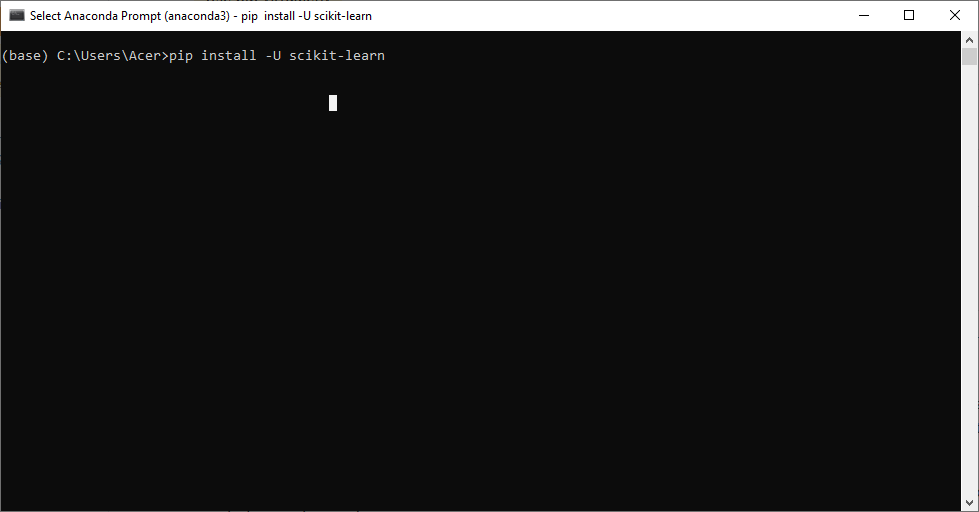
\includegraphics[scale=0.4]{figures/1.PNG}
		
	\end{figure}
\newpage
\item
Mencoba Loading an example dataset, menjelaskan maksud dari tulisan tersebut dan mengartikan per baris[hari ke 1](10)
\begin{figure}[!htbp]
		\centering
		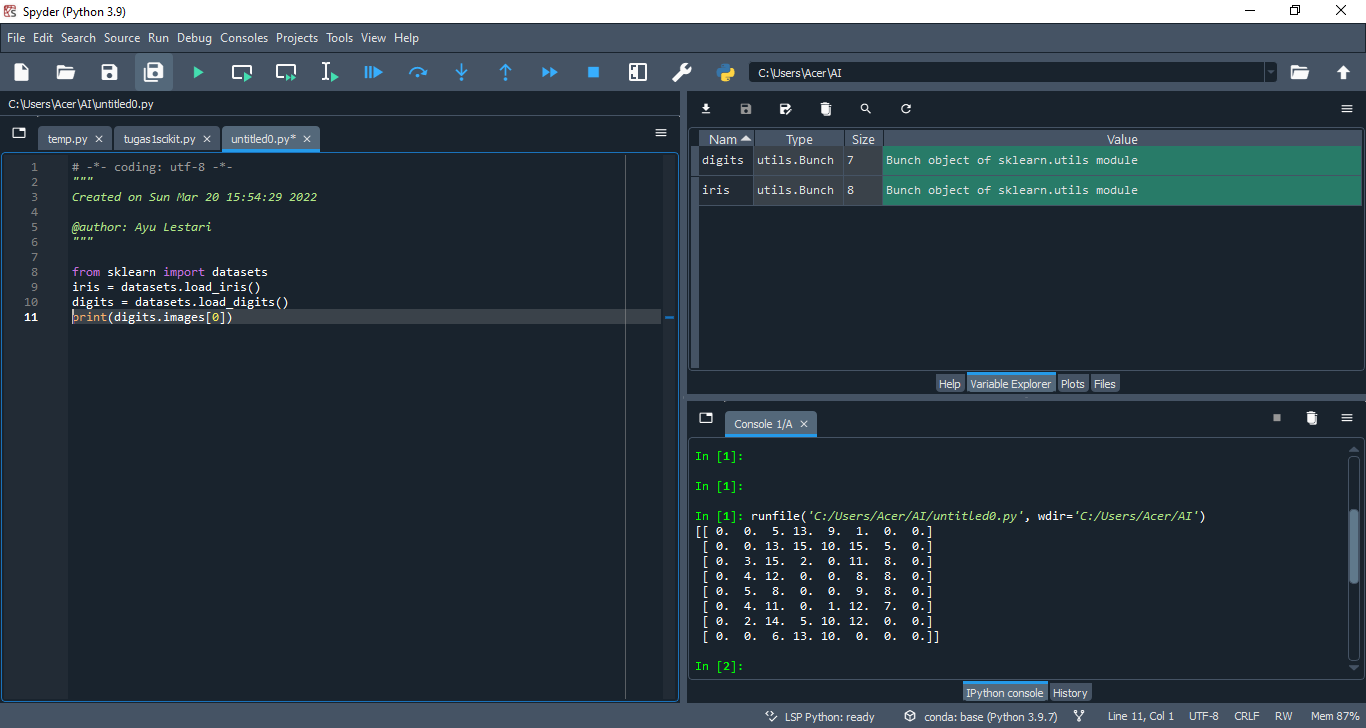
\includegraphics[scale=0.4]{figures/2.PNG}
	
	\end{figure}
\newpage
\item
Mencoba Learning and predicting, menjelaskan maksud dari tulisan tersebut dan mengartikan per baris[hari ke 2](10)
\begin{figure}[!htbp]
		\centering
		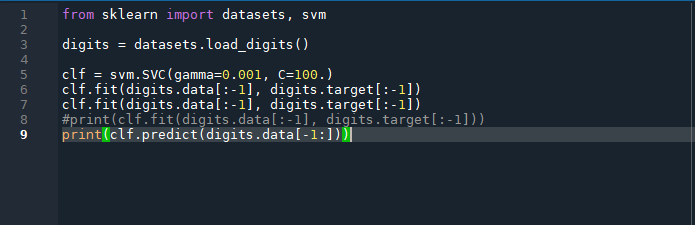
\includegraphics[scale=0.4]{figures/3.PNG}
	
	\end{figure}
\newpage
\item
mencoba Model persistence, menjelaskan maksud dari tulisan tersebut dan mengartikan per baris[hari ke 2](10)
\begin{figure}[!htbp]
		\centering
		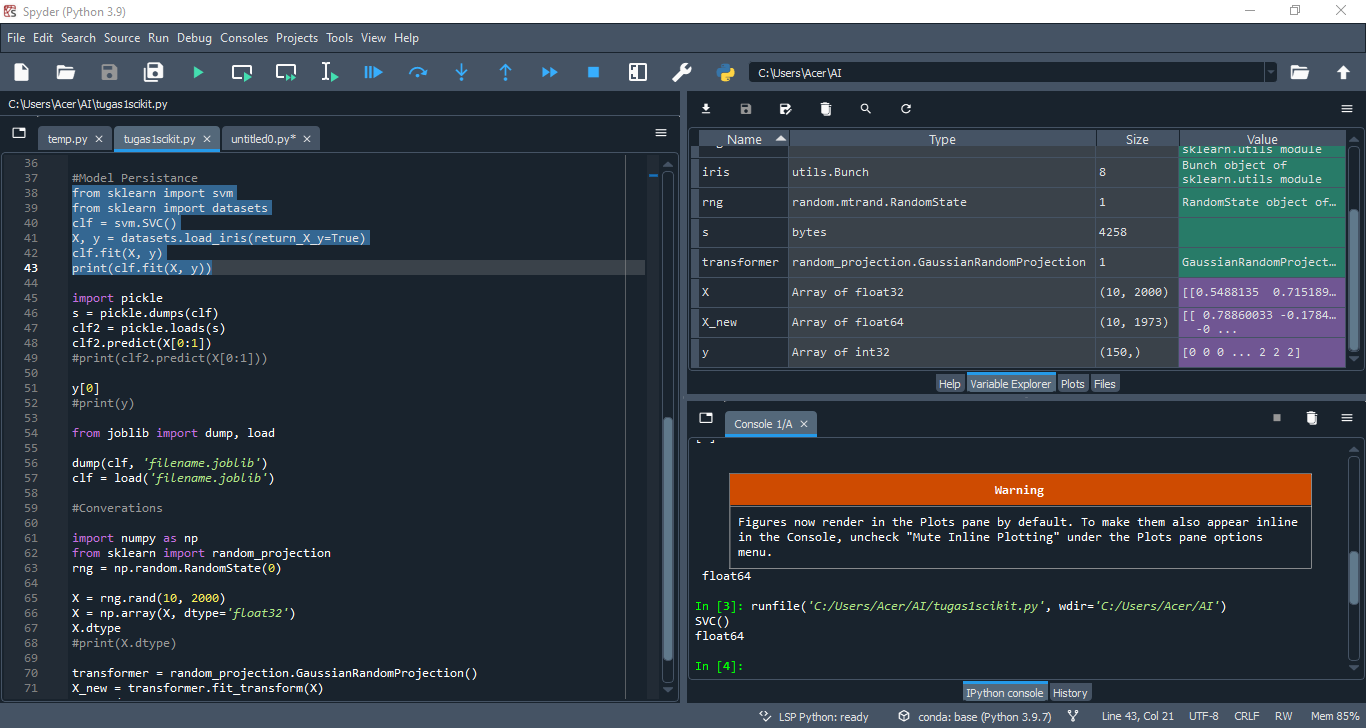
\includegraphics[scale=0.4]{figures/4.PNG}
	
	\end{figure}
\newpage
\item 
Mencoba Conventions, menjelaskan maksud dari tulisan tersebut dan mengartikan per baris[hari ke 2](10)
\begin{figure}[!htbp]
		\centering
		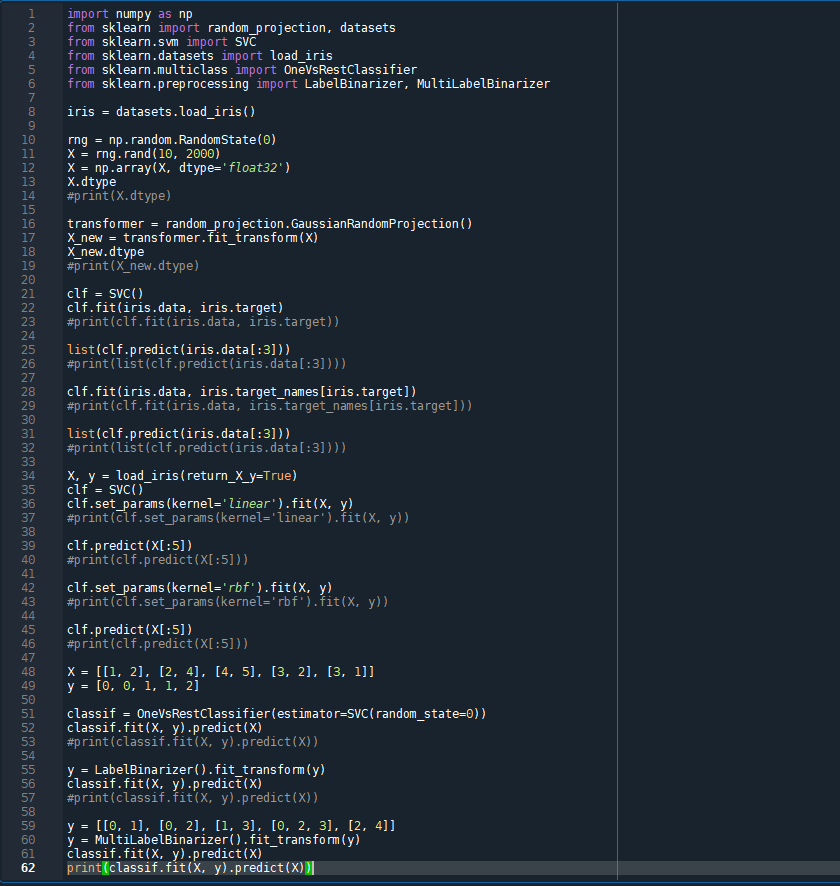
\includegraphics[scale=0.4]{figures/5.PNG}
		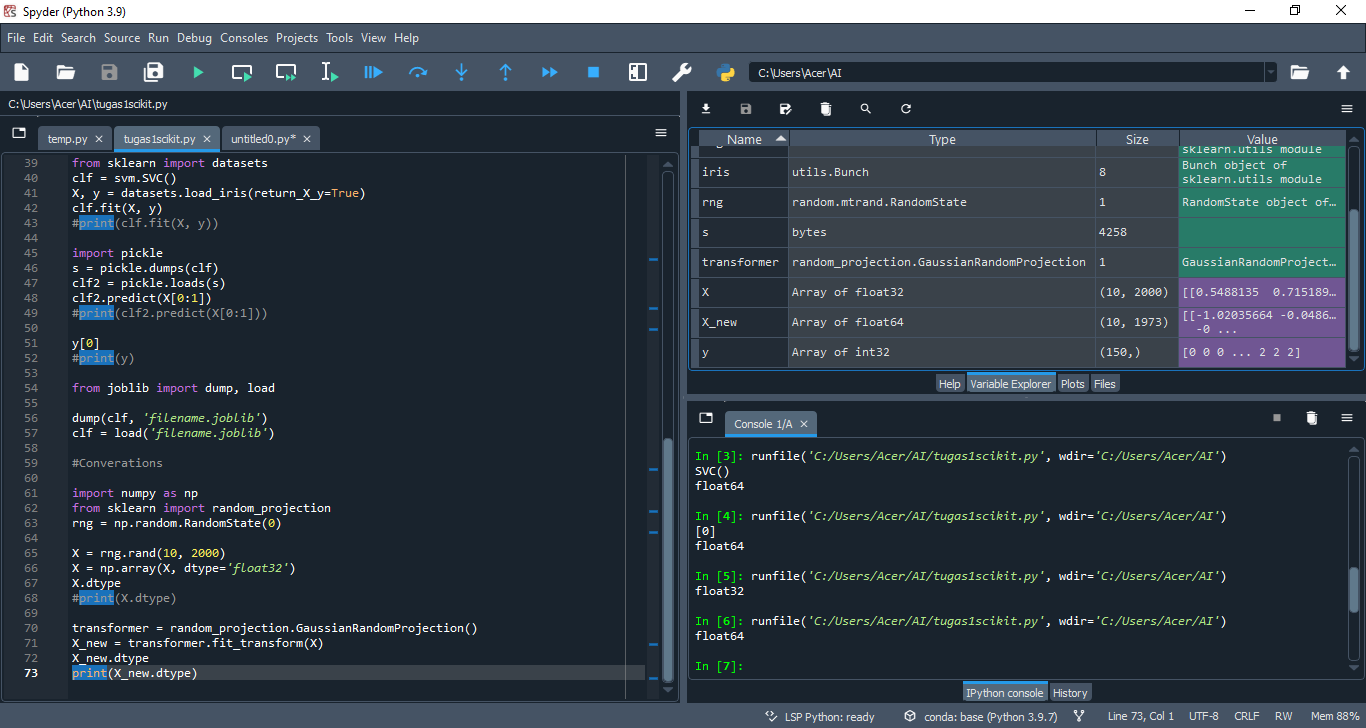
\includegraphics[scale=0.5]{figures/6.PNG}
	\end{figure}
\newpage
\end{enumerate}


\section{Penanganan Error}
Dari percobaan yang dilakukan di atas, apabila mendapatkan error maka:

\begin{enumerate}
	\item
	skrinsut error[hari ke 2](10)
	\item
Tuliskan kode eror dan jenis errornya [hari ke 2](10)
	\item
Solusi pemecahan masalah error tersebut[hari ke 2](10)

\end{enumerate}



